\documentclass[14pt]{beamer}
%\documentclass[14pt,handout]{beamer}

\setbeamercolor{item projected}{bg=black}
\setbeamertemplate{itemize items}[circle]
\graphicspath{{Figures/}}
\mode<presentation>
{
%  \usetheme{Boadilla}
  \usetheme{CambridgeUS}
  % or ...

  \setbeamercovered{transparent}
  % or whatever (possibly just delete it)
}


%\usepackage[english]{babel}
% or whatever

%\usepackage[latin1]{inputenc}
% or whatever
\usepackage{amsmath,amssymb,latexsym,epsfig,graphicx,psfrag,pstricks, fancybox, ulem}
\usepackage{booktabs}
%\title{Seminar Presentation} % (optional, use only with long paper titles)
\subtitle{Modelling and analysis of a financial market with slow and fast trading agents acting on time-delayed market information}
\title{Master's Thesis}
\author{Halfdan Rump}
\date{February 5 2014} % (optional, should be abbreviation of conference name)
\institute{Waseda GRS-FSE} % (optional, but mostly needed)

\newenvironment{changemargin}[2]{% 
  \begin{list}{}{% 
    \setlength{\topsep}{0pt}% 
    \setlength{\leftmargin}{#1}% 
    \setlength{\rightmargin}{#2}% 
    \setlength{\listparindent}{\parindent}% 
    \setlength{\itemindent}{\parindent}% 
    \setlength{\parsep}{\parskip}% 
  }% 
  \item[]}{\end{list}} 



\begin{document}

\begin{frame}
  \titlepage
\end{frame}





\section{Introduction}
\begin{frame}
\tableofcontents[currentsection]
\end{frame}

\begin{frame}{Background and motivation}
A few fact about modern financial markets:
\begin{itemize}
	\item Humans trade against software algorithms (the machines) 
	\item Humans are slow but complex, whereas algorithms are fast, but (relatively) simple
	\item Fast crashes (flash crashes) has become a problem in recent years
\end{itemize}
\end{frame}

\begin{frame}{Related work}
Models for human/machine system must be developed. Previous work:
\begin{description}
	\item[Analysis of market data] Works analyzing real market data for flash crashes and
	\item[Models of markets] Works that divide agents into two groups: \textbf{slow} and \textbf{fast} traders
\end{description}
All discovered works in the field are recent (published 2013, or yet unpublished).
\end{frame}

\begin{frame}{Key ideas in proposed model}
\begin{description}
\item[Delayed market information] All information exchanged between agents and the market is delayed
\item[Agents with arbitrary time delays] Agents are not just \textit{fast} or \textit{slow}, but have \textbf{arbitrary} delays
%\i tem[Full-fledged MAS model] Agents with various strategies and different delays.
\end{description}
\end{frame}

\begin{frame}{Research goal}
\begin{block}{Impact of agent speed on market behavior}
Investigate how the behavior (e.g. stable, crash, etc.) of a simulated financial market changes when the latency of the traders change
\end{block}
%Very open research, but the first steps in a new field must necessarily be somewhat exploratory.
\end{frame}


%\begin{frame}{Methodology}
%
%\begin{itemize}
%content...
%\end{itemize}
%\end{frame}






\section{Model}
\begin{frame}
\tableofcontents[currentsection]
\end{frame}

\begin{frame}{Market model}
\begin{columns}[c]
\column{2.5in}
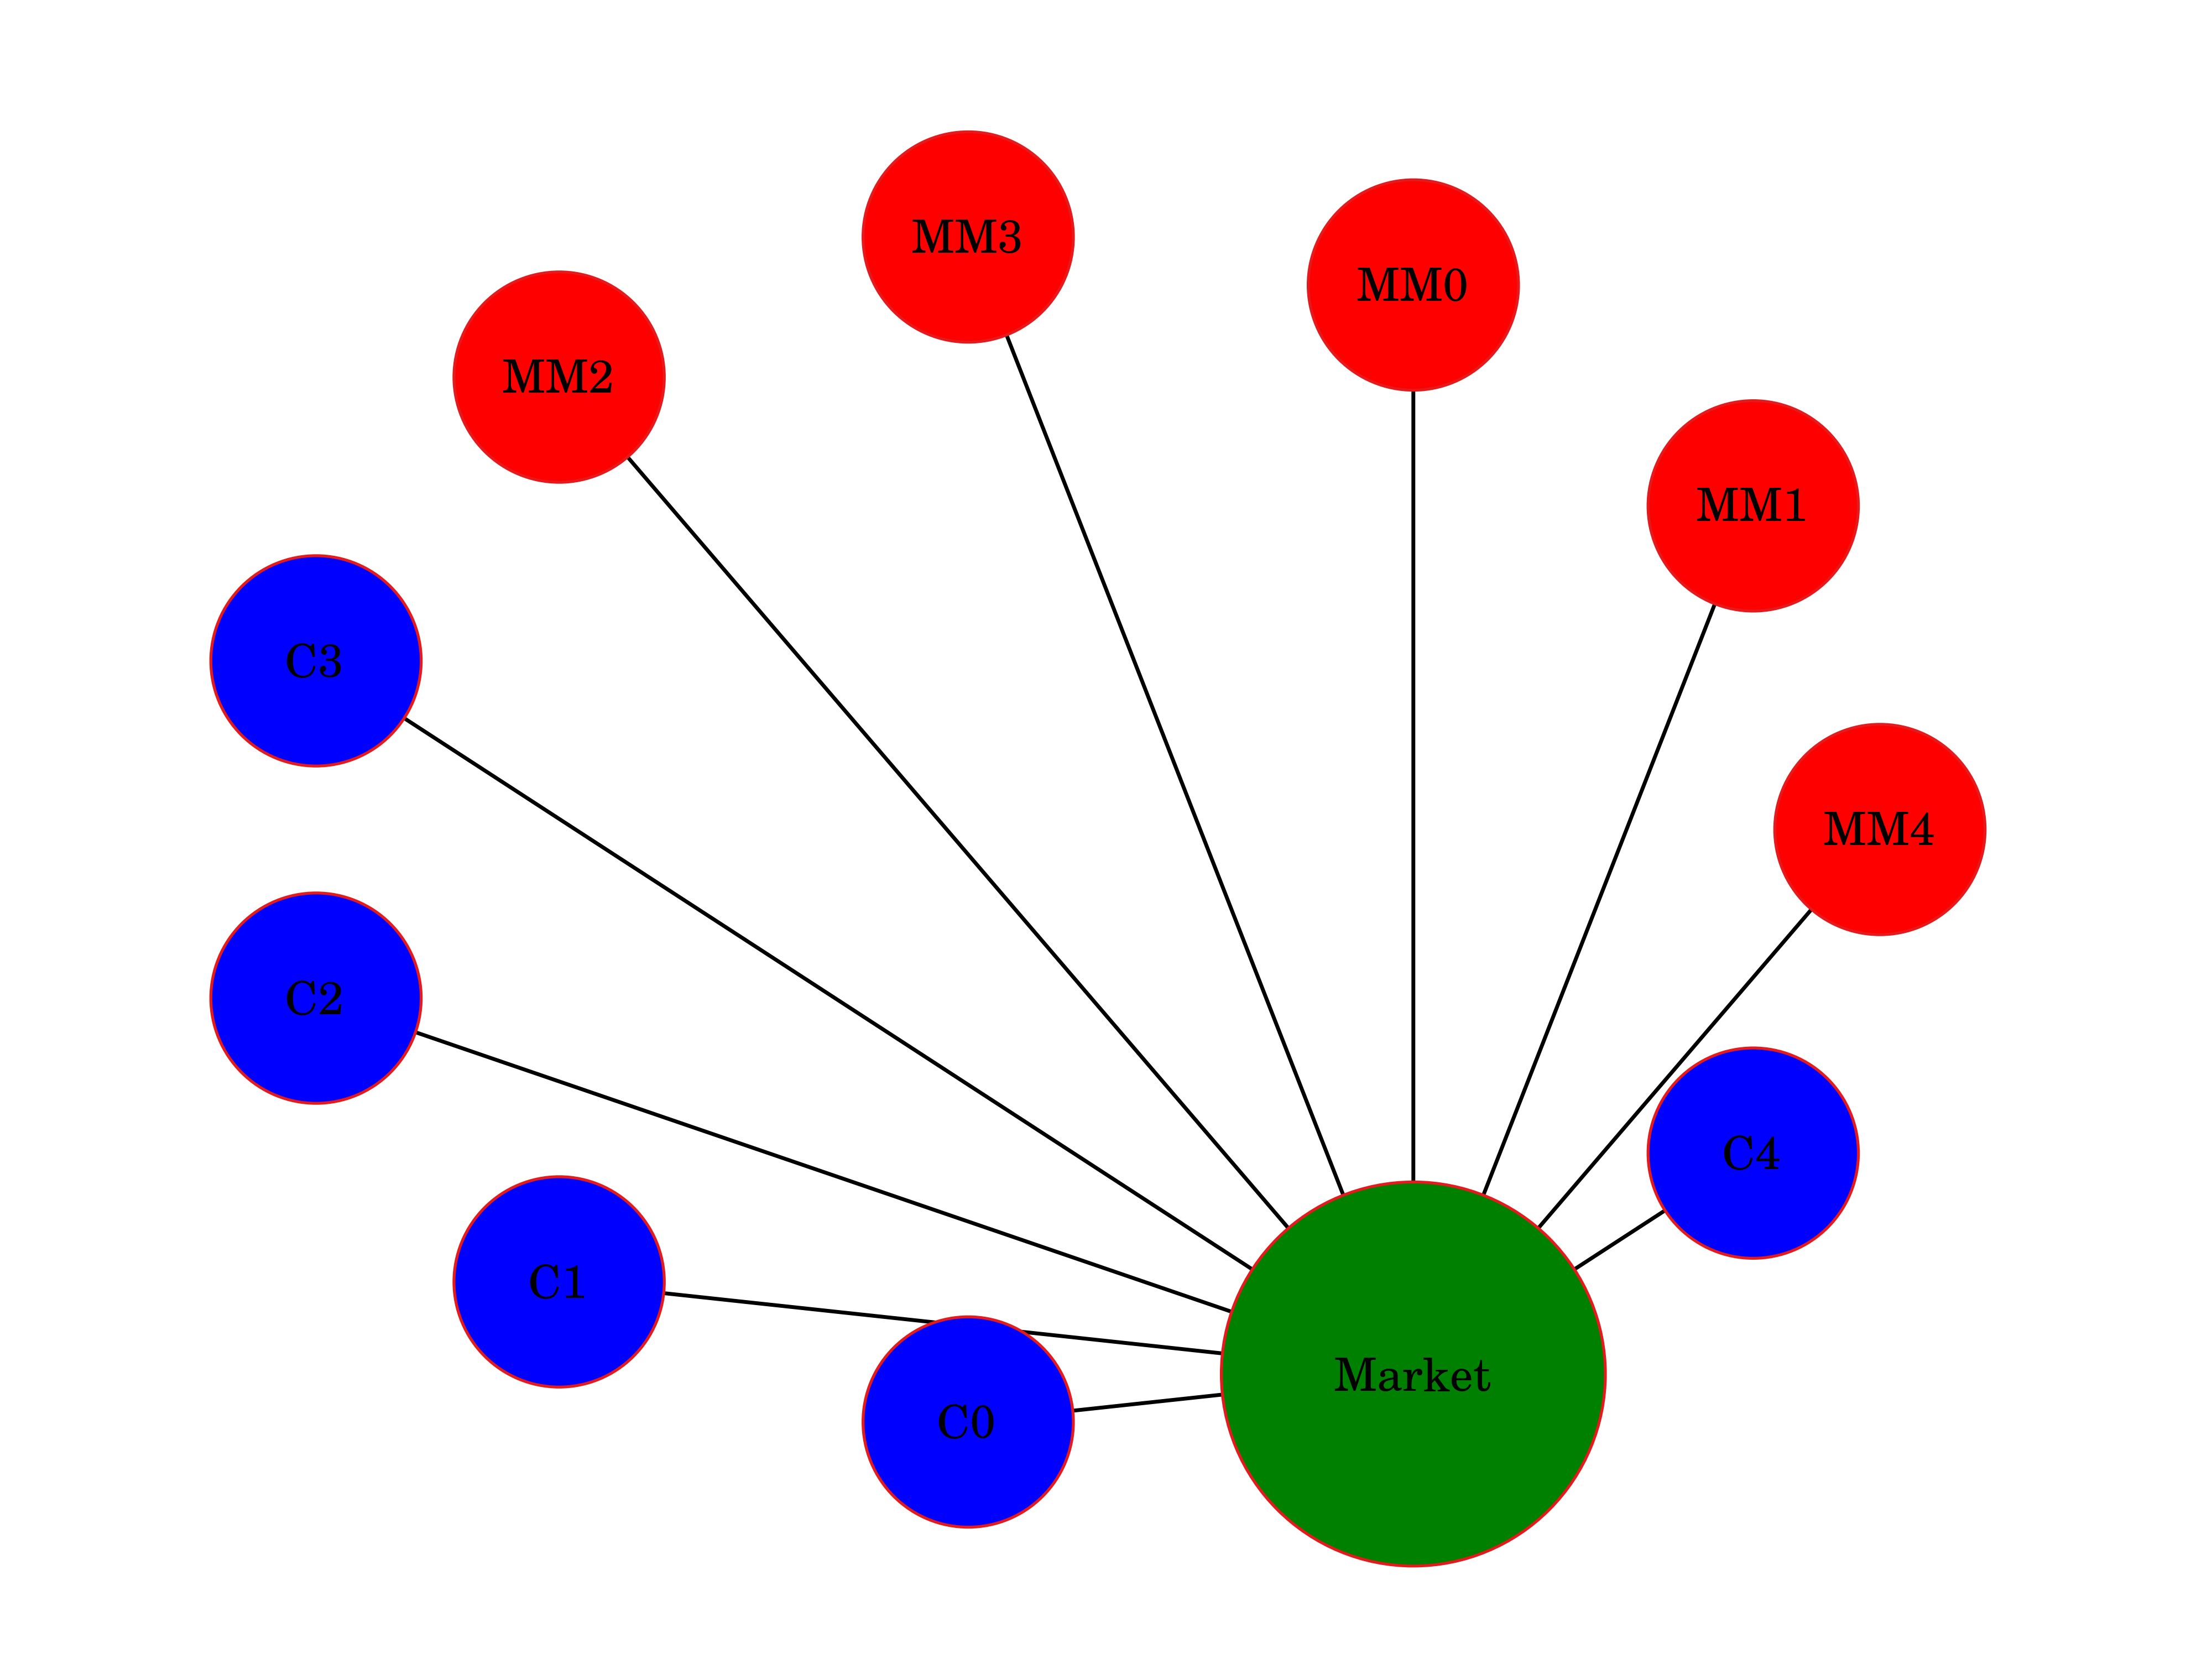
\includegraphics[width=1.2\textwidth]{graph.png}
\column{2in}
Model components:
\begin{itemize}
\item Market
\item Stock
\item Agents
\item Messages (orders, cancellations, receipts, etc.)
\end{itemize}
\end{columns}
\pause
\underline{Messages are passed between agents and the market.}
\end{frame}


\begin{frame}{Messages are delayed}
Information travels from agents to market in different kinds of messages
\begin{itemize}
\item Market information
\item Orders
\item Receipts
\item Cancellations
\end{itemize}
\textit{All messages have a non-zero travel time}
\end{frame}

\begin{frame}{Stock}
A single stock is traded at the market.
\begin{description}
\item[Fundamental price] The ``\textit{true}'' value of the stock
\item[Traded price] The price at which the stock is currently traded
\end{description}
\end{frame}


\begin{frame}{Agents}
\begin{itemize}
\item Slow traders
\vspace{0.1in}
\item Fast traders (High Frequency Traders)
\begin{itemize}
\item Market makers
\item Simple chartists
\end{itemize}
\end{itemize}
\end{frame}



\begin{frame}{Slow traders}
\begin{block}{Slow traders model human traders}
They know the \textbf{true} value of the fundamental, \textit{but with a large delay}
\end{block}
\vspace{0.1in}
The slow traders submit orders in order to \textit{move the trade price towards the true price}.
\end{frame}


%\begin{frame}{Simple chartists}
%\begin{block}{The chartists use a simple moving average strategy}
%They calculate the moving from the delayed best buy and sell prices. 
%\end{block}
%The chartist detects a trend if the moving average calculated over $H_c$ rounds differs more than $\gamma_c$ ticks f %rom the currently traded price.
%\end{frame}

%\begin{frame}{Chartist example 1}
%\begin{center}
%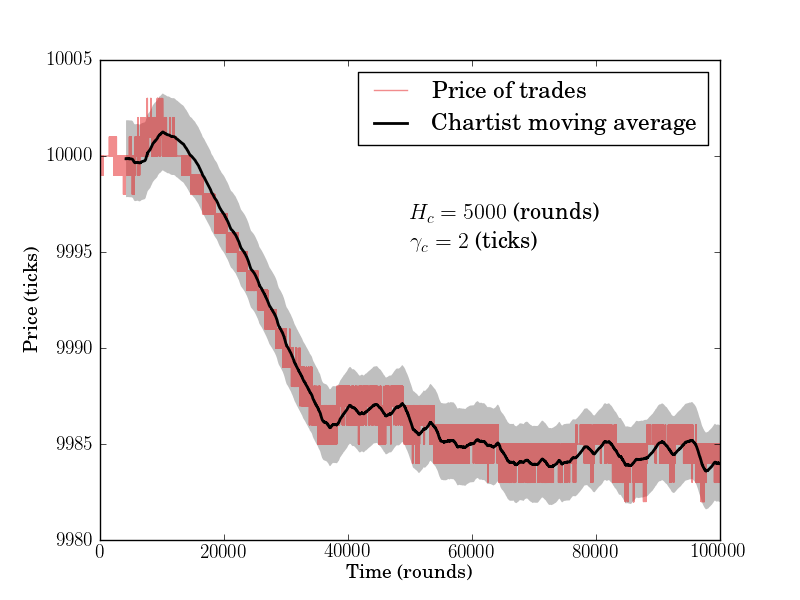
\includegraphics[width=0.7\textwidth]{chartist/b.png}
%\end{center}
%\end{frame}

\begin{frame}{Fast trader: simple chartist}
The chartists use a simple moving average strategy:
\begin{center}
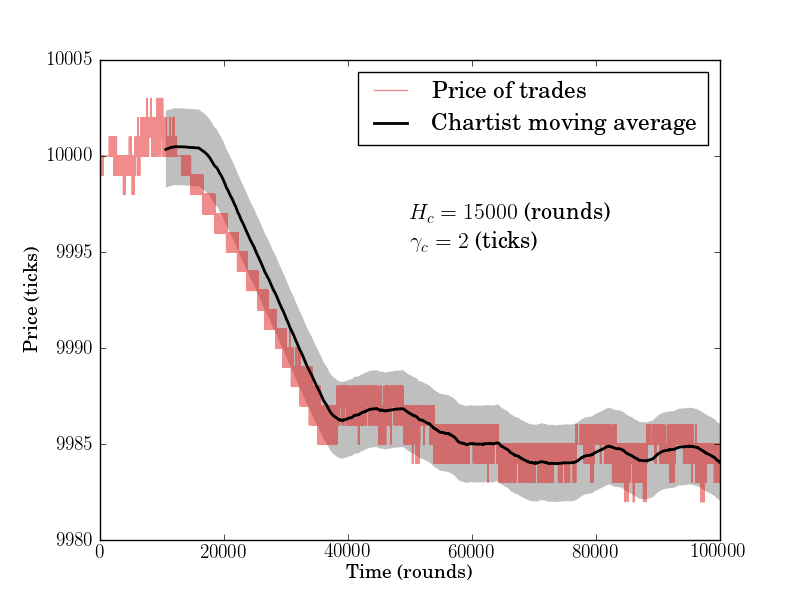
\includegraphics[width=0.7\textwidth]{chartist/h.png}
\end{center}
\end{frame}



%\begin{frame}{Market makers}
%\begin{block}{Market makers keep constant buy and sell orders}
%The market maker tried to follow the best buy/sell prices to stay competitive.
%\end{block}
%The market maker has a minimum-spread parameter, $\theta$.
%\end{frame}

\begin{frame}{Market maker case}
Market makers try to keep constant orders at both sides of the book.
\begin{center}
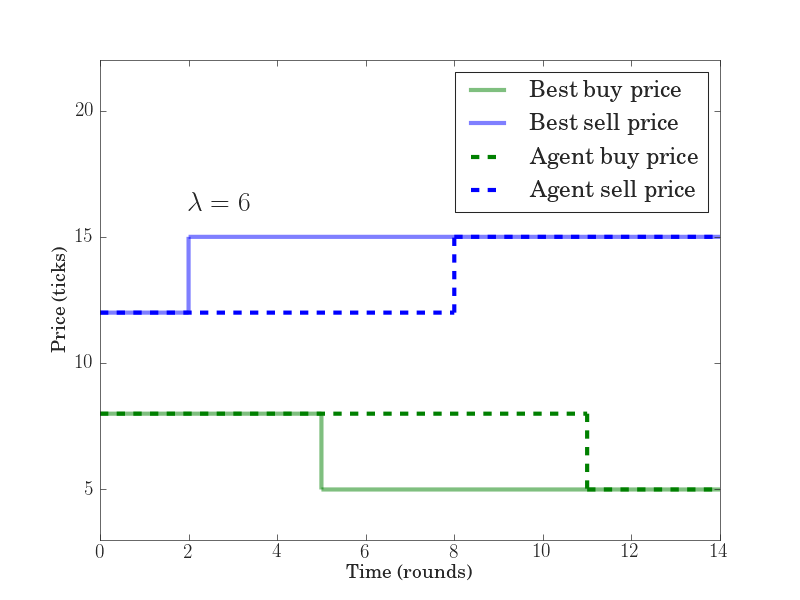
\includegraphics[width=0.7\textwidth]{marketmaker/a.png}
\end{center}
\end{frame}


\begin{frame}{Model recap}
\begin{itemize}
\item \textit{Any} exchange of information between the market and agents is time delayed.
\vspace{0.1in}
\item Agent speeds are \textit{quantitative} (e.g., 11 rounds or 23 rounds), instead of \textit{qualitative} (slow or fast) as in previous models
\end{itemize}
\end{frame}

\section{Experiments}
\begin{frame}
\tableofcontents[currentsection]
\end{frame}

%\begin{frame}{Important model parameters}
%The model has many parameters. The most important ones are:
%\begin{itemize}
%\ item The average latency of chartists and of market makers, $\lambda$
%\item The ``power balance'' between the agents. 
%\end{itemize}
%\end{frame}

\begin{frame}{Simulating bad news}
How does the market react when the true price of the stock suddenly drops?
\begin{center}
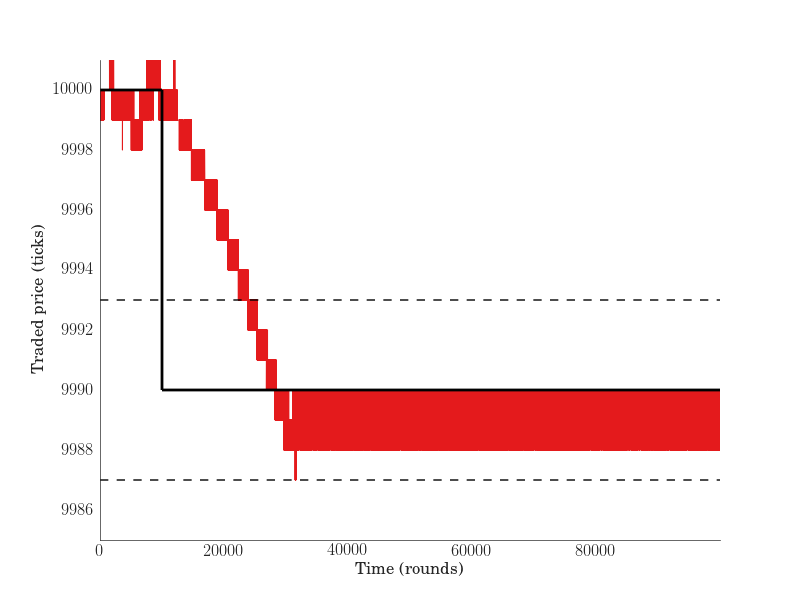
\includegraphics[width=0.7\textwidth]{market_cases/a_stable_within_margin.png}
\end{center}
\end{frame}

\begin{frame}{Exploring model behavior with inverse simulation}
A genetic algorithm was used to find parameters causing \textbf{stable markets}. Four measures for model fitness were defined:
\pause
\begin{small}
\begin{description}
\item[Overshoot] Used to find \textbf{market crashes}
\item[Response time] Used to measure market reaction speed to \text{bad news}
\item[Price flickering] Standard deviation of trade prices)
\item[Time to become stable] the traded price must stay within a certain range of the true price)
\end{description}
\end{small}
\end{frame}

\begin{frame}{Stable market}
Stable markets are found by minimizing all four fitness measures
\begin{center}
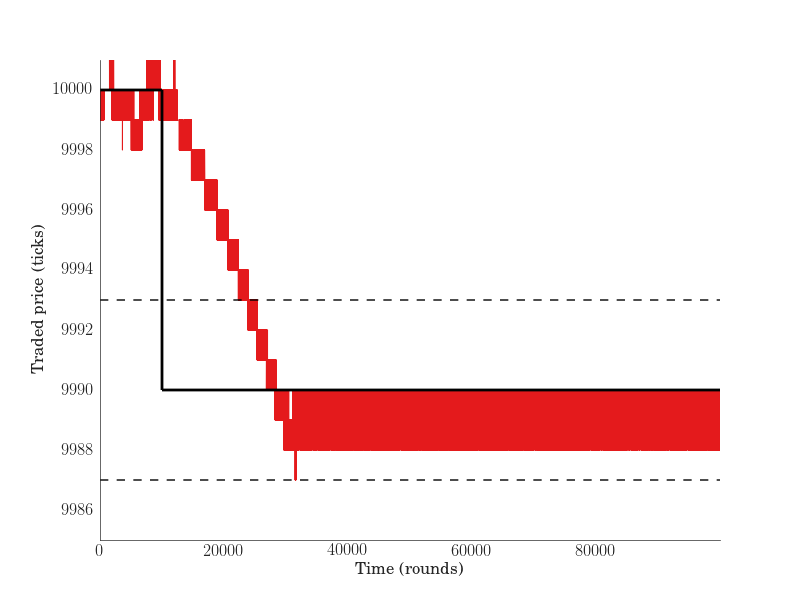
\includegraphics[width=0.6\textwidth]{market_cases/a_stable_within_margin.png}
\end{center}
\pause
Small overshoot, little price flickering
\end{frame}

\begin{frame}{Market with large price flicker}
\begin{center}
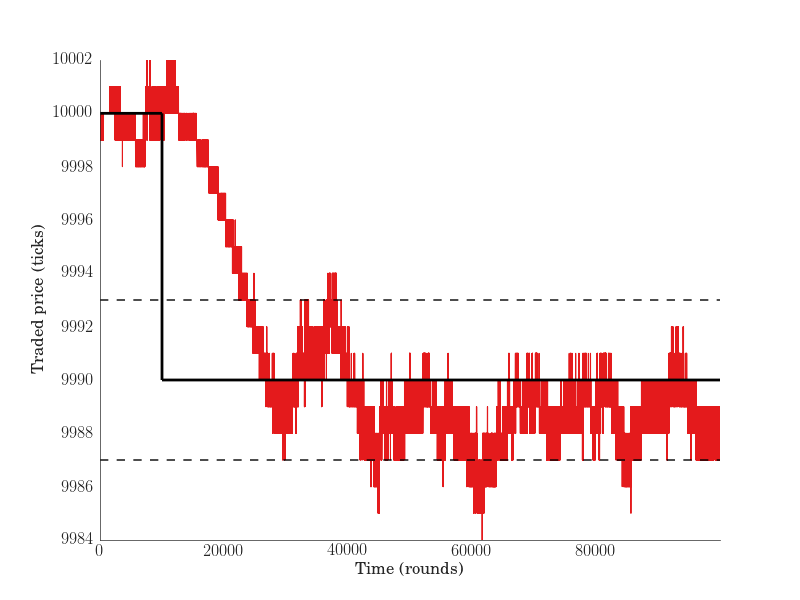
\includegraphics[width=0.6\textwidth]{market_cases/b_flicker_but_mostly_within_margin.png}
\end{center}
Small overshoot but large price flickering.
\end{frame}
 
\begin{frame}{Market crash}
Crashing markets can be found by maximizing the overshoot.
\begin{center}
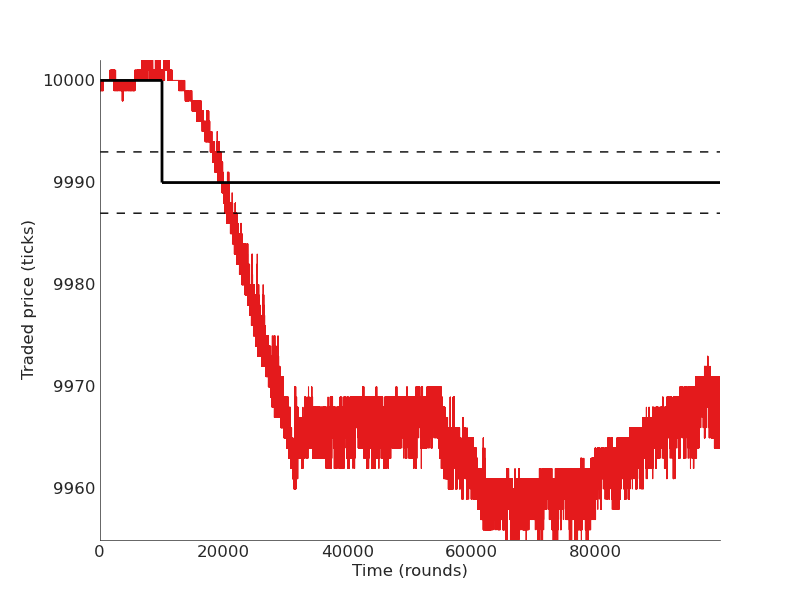
\includegraphics[width=0.7\textwidth]{market_cases/f_crash.png}
\end{center}
\end{frame}







	
\section{Results}


\begin{frame}
\tableofcontents[currentsection]
\end{frame}
\subsection{Speed/stability trade-off}

\begin{frame}{Speed/stability trade-off}
\begin{itemize}
\item Stable markets are slow
\item Slow markets are stable
\end{itemize}
What parameters cause this behavior?
\end{frame}



\begin{frame}{Speed/stability trade-off}
The GA found \color{red} stable markets \color{black} (i.e.,\textit{small overshoot})
\begin{center}
\includegraphics[width=0.6\textwidth]{evolution/overshoot_ellipse.png}
\end{center}
\end{frame}

\begin{frame}{Speed/stability trade-off}
... but the markets were \color{red} unresponsive \color{black} (i.e., \textit{slow to reach the new fundamental price})
\begin{center}
\includegraphics[width=0.6\textwidth]{evolution/time_to_reach_new_fundamental_ellipse.png}
\end{center}
\end{frame}




\subsection{Agent speed and market stability}
\begin{frame}
\tableofcontents[currentsubsection]
\end{frame}


\begin{frame}{Research goal recap 1}
\begin{block}{Central question}
How does the \color{red} fast trader speed \color{black} affect the \textit{market stability}?
\end{block}
\vspace{0.2in}
\pause
\textit{E.g., do faster traders make the markets unstable?}
\end{frame}

\begin{frame}{Chartist speed and market stability}
\begin{columns}[c]
\column{2in}
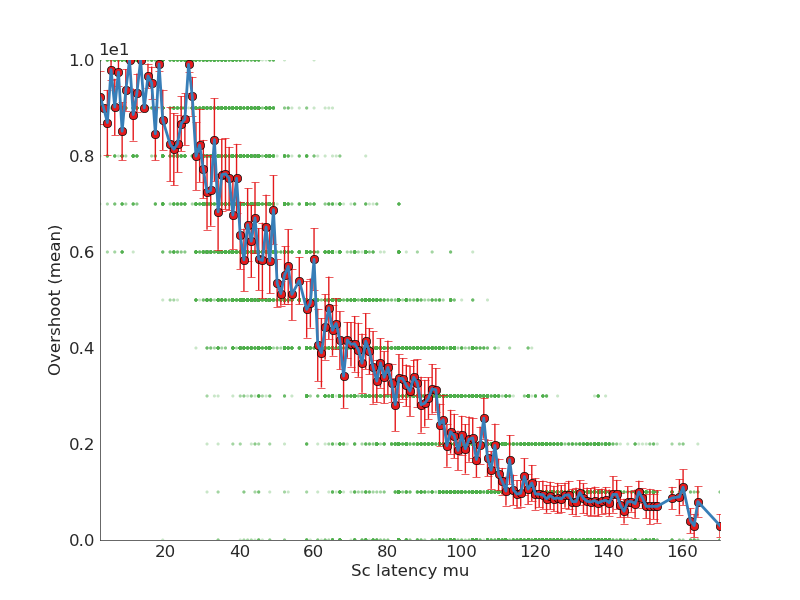
\includegraphics[width=1.3\textwidth]{scatter/sc_latency_mu__vs__overshoot(mean)_scatter.png}
\column{1.5in}
%\begin{itemize}
\color{red} Faster chartists \color{black} cause the market to have a \color{red} larger overshoot\color{black} (i.e. the market becomes \textit{unstable}).
%\item In some markets with \textbf{very fast} chartists, the market \color{red} crashes \color{black}.
%\end{itemize}
\end{columns}
\end{frame}

\begin{frame}{Market maker speed and market stability}
\begin{columns}[c]
\column{2in}
\includegraphics[width=1.3\textwidth]{scatter/ssmm_latency_mu__vs__overshoot(mean)_scatter.png}
\column{1.5in}
\color{red} Faster market makers \color{black} cause the market to have a \color{red} somewhat \color{black} larger overshoot \textit{in some cases}.
\end{columns}
\end{frame}

%\begin{frame}{Number of chartists}
%...as has the number of chartists:
%\begin{center}
%\ includegraphics[width=0.7\textwidth]{scatter/sc_nAgents__vs__overshoot(mean)_scatter.png}
%\end{center}
%\end{frame}

\subsection{Relative speed and market stability}
\begin{frame}
\tableofcontents[currentsubsection]
\end{frame}

\begin{frame}{Research goal recap 2}
\begin{block}{Central question}
Does the \color{red} relative speed \color{black} of the fast traders matter to market stability, and if so \textit{how}?
\end{block}
\vspace{0.2in}
\pause
\textit{E.g., what happens when the chartists are faster than the market makers, or the other way around?}
\end{frame}


\begin{frame}{Relative trader speed and market crashes}
\begin{columns}
\column{1.7in}
\includegraphics[width=1.5\textwidth]{ratio/overshoot_wt.png}
\column{1.7in}
\begin{itemize}
\item \color{blue} \textbf{Stable markets} \color{black} had \textbf{few} and \textbf{slow} chartists
\item \color{red} \textbf{Market crashes}\color{black}\ happened with \text{many} and \textbf{fast} chartists
\end{itemize}
\end{columns}
\end{frame}


%\begin{frame}{Log-overshoot}
%\begin{center}
%\ includegraphics[width=0.7\textwidth]{ratio/overshoot_log.png}
%\end{center}
%\end{frame}

\begin{frame}{Relative trader speed and response time}
\begin{columns}
\column{1.7in}
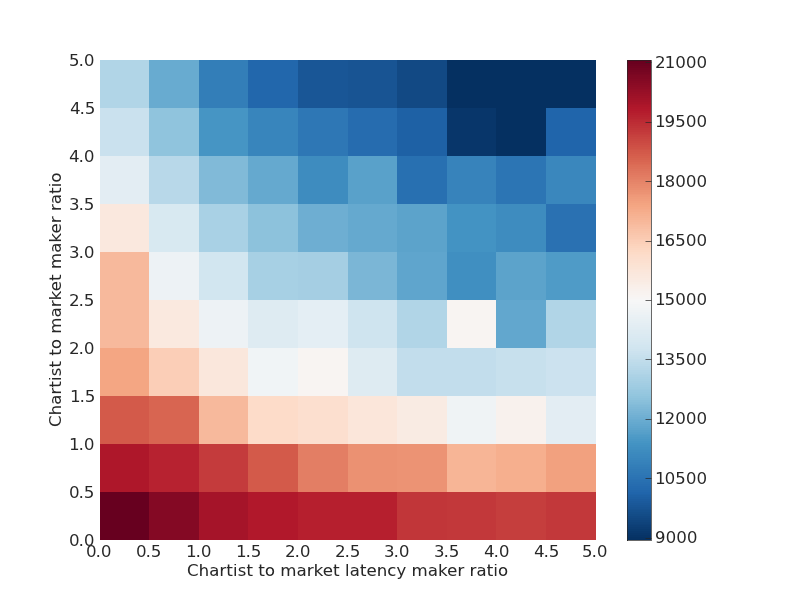
\includegraphics[width=1.5\textwidth]{ratio/time_to_reach_new_fundamental.png}
\column{1.7in}
\begin{itemize}
\item \color{red} \textbf{Unresponsive}\color{black}\ market had \text{few} and \textbf{slow} chartists
\item \color{blue} \textbf{Responsive} \color{black} markets had \textbf{many} and \textbf{fast} chartists
\end{itemize}
\end{columns}
\end{frame}

\subsection{Summary of results}
\begin{frame}
\tableofcontents[currentsubsection]
\end{frame}

\begin{frame}{Agent speed is important}
\begin{enumerate}
\item Market makers \color{green} \textbf{increase stability} \color{black} the market, but \color{red} \textbf{decrease responsiveness} \color{black}.
\vspace{0.1in}
\pause
\item Chartists \color{green} \textbf{increase responsiveness} \color{black}, but \color{red} \textbf{decrease stability} \color{black}
\end{enumerate}
\vspace{0.2in}
\pause
\begin{center}
\large
\underline{The influence was \textit{larger} for \textit{faster} agents}
\end{center}
\end{frame}

\begin{frame}{Conditions for market crashes}
\begin{enumerate}
\item The market \textit{may} \color{red} crash \color{black} when there are \textbf{many fast} chartists, but \textbf{only} if there are also \textit{some} active of market makers \vspace{0.1in} \pause
\item The market was more likely to crash if the \textit{chartists were faster than the market makers}
\end{enumerate}
\end{frame}


\section{Conclusion}
\begin{frame}
\tableofcontents[currentsection]
\end{frame}

\begin{frame}{Conclusion}
Fast traders are both good and bad for the market:
\begin{itemize}
\item Fast traders can \color{green} \textbf{reduce misvaluation} \color{black}, but also cause \color{red} \textbf{market crashes}. \color{black}
\end{itemize}
\vspace{0.2in}
\pause
Modeling relative speed of different agents can give new insights
\begin{itemize}
\item Market crashes did not just happen with many fast traders, but when some fast trader were \textbf{faster} than others.
\end{itemize}
\end{frame}

\begin{frame}
\begin{center}
\Large
Thank you for your attention.
\end{center}
\end{frame}





\begin{thebibliography}{Selected bibliography}
\scriptsize
\bibitem{mcgowan}
  Michael, J. McGowan,
  \emph{The Rise of Computerized High Frequency Trading: Use and Controversy}.
  Duke Law \& Technology Review,
  2012.
 \bibitem{izumi}
  K. Izumi, F. Toriumi, H. Matsui
  \emph{Evaluation of automated strategies using an artificial market}.
  Neurocomputing,
  2009.
  \bibitem{cincotti}
  S. Cincotti, S.M. Focardi, L. Ponta, M. Raberto, E. Scalas
  \emph{The waiting-time distribution of trading activity in a double auction artificial financial market}. Unpublished, 2011
  \bibitem{luca}
  M. De Luca, C. Szostek, J. Cartlidge, D. Cliff
  \emph{Studies of interactions between human traders and algorithmic trading systems}.
  Commissioned as part of the UK {Government's} Foresight Project, The Future of Computer Trading in Financial Markets--Foresight Driver Review--DR 13, 2011
  \bibitem{johnson}
  N. Johnson, G. Zhao, E. Hunsader, J. Meng, A. Ravindar, S. Carran, B. Tivnan
  \emph{Financial black swans driven by ultrafast machine ecology}.
  Submitted, 2012.
\end{thebibliography}



\end{document}


